\section{Types of Verification}


\subsection{Functional Verification With Strip, Bind, and Search}
A typical large building contains thousands of sensors, monitoring the HVAC system, lighting, and other operational sub-systems.
With the increased push for operational efficiency, operators are relying more on historical data processing to uncover opportunities for energy-savings.
However, they are overwhelmed with the deluge of data and seek more efficient ways to identify potential problems.
In this paper, we present a new approach called the Strip, Bind and Search (SBS); a method for uncovering abnormal 
equipment behavior and in-concert usage patterns.
SBS uncovers relationships between devices and constructs a model for their usage pattern relative to other devices.
It then flags deviations from the model. 
% Unlike other approaches, SBS requires no a priori knowledge about the building.
We run SBS on a set of building sensor traces; each containing hundred sensors reporting data flows over 18 weeks from two separate buildings with fundamentally different infrastructures.  
We demonstrate that, in many cases, SBS uncovers misbehavior corresponding to inefficient device usage that leads to energy waste.  
The average waste uncovered is as high as 2500~kWh per device. 

The intuition behind the proposed approach is that each service provided by the building requires a minimum subset of devices.
The devices within a subset are used at the same time when the corresponding service is needed and a savings opportunity is characterized by the partial activation of the devices.
For example, office comfort is attained through sufficient lighting, ventilation, and air conditioning.
These are controlled by the lighting and HVAC (Heating, Ventilation, and Air Conditioning) system.
%controlled by the lighting system and air conditioner.% the light and air conditioning.
Thus, when the room is occupied both the air conditioner (heater on a cold day) and lights are used together and should be turned off 
when the room is empty.
In principal, if a person leaves the room and turns off \emph{only} the lights then the air conditioner (or heater) is a source of electricity waste.

Following this basic idea we propose \emph{Strip, Bind and Search} (SBS), an unsupervised methodology that systematically detects electricity waste.
Our proposal consists of two key components:
% \begin{enumerate}
%  \item The strip and bind method (SBM) mines raw sensor data, identifying devices that are used in concert.
%  It uncovers the devices relationships by looking at the correlation of their activities. 
%  Therefore it allows us to differentiate the devices that are used all together (high correlation), devices used independently (no correlation) and the mutually exclusive usages of devices (negative correlation).
%  \item The anomaly detector monitors devices relationships over time and reports misbehaving devices.
%  It learns the devices normal usages using a robust and longitudinal analysis of the building data and detect anomalous usages that stand for electricity wastes.
% \end{enumerate}

\begin{description}
 \item[Strip and Bind] The first part of the proposed method mines the raw sensor data, identifying inter-device usage patterns. % that are typically used in concert to provide a service.
We first \emph{strip} the underlying traces of occupancy-induced trends.  Then we \emph{bind} devices  whose underlying behavior is highly correlated. %, by placing them into a correlated device set.
 %  Then
 % It uncovers the devices relationships by looking at the correlation of their activities. 
 This allows us to differentiate between devices that are used together (high correlation), used independently (no correlation), and used mutually exclusively (negative correlation).
 \item[Search] The second part of the method monitors devices relationships over time and reports deviations from the norm.  % misbehaving devices.
 It learns the normal inter-device usage using a robust, longitudinal analysis of the building data and detect anomalous usages.  Such abnormalities usually present an opportunity to reduce electricity waste or events that deserve careful attention (e.g. faulty device).
 % that may represent that stand for electricity wastes.
\end{description}

SBS overcomes several challenges.  First, 
%The main challenge we overcame with our approach is uncovering the device relationships from numerous, 
noisy sensor traces that all share a similar trend, making direct correlation analysis non-trivial.
%The main difficulty in this approach is to uncover the devices relationship from the numerous and noisy sensor traces. 
Device energy consumption is mainly driven by occupancy and weather, all the devices display a similar daily pattern, in 
roughly overlapping time intervals and phases.
%and seem to be used all at once.
Therefore, one of the main contributions of this work is uncovering the intrinsic device relationships by filtering out the 
dominant trend.  For this task we use 
%% Romain
%This is achieved using a signal processing technique that exhibit the inherent characteristics of time series data, the 
Empirical Mode Decomposition \cite{huang:emd1998}, a known method for de-trending time-varying signals.
%% Romain

Another key contribution of this work is in using SBS to practically monitor building energy consumption.
Moreover, the proposed method is easy to use and functions in any building, as it does not require prior knowledge of the building nor extra sensors.  
It is also tuned through a single intuitive parameter.  %which parameter?

We validate the effectiveness of our approach using 10 weeks of data from a modern Japanese building containing 135 sensors and 
8 weeks of data from an older American building containing 70 sensors.
These experiments highlight the effectiveness of SBS to uncover device relationships in a large deployment of 135 sensors.
Furthermore, we inspect the SBS results and show that the reported alarms correspond to significant opportunities to save energy.
The major anomaly reported in the American building lasts 18 days and accounts for a waste of 2500 kWh. % for a single device whereas the building average power consumption is 600 kW per hour.
% SBS also reported numerous smaller anomalies that are hidden in the building's overall consumption, thus, difficult for building operators to identify without the proposed method.
SBS also reports numerous small anomalies, hidden deep within the building's overall consumption data.  Such errors are very difficult to find
without SBS.

In the rest of this paper, we detail the mechanisms of SBS (Section \ref{methodo}) before evaluating it with real data (Section \ref{eval}) then we discuss different outcomes of the proposed methodology (Section \ref{discussion}) and conclude.


\subsection{Spatial Verification}

We investigate the utility of empirical mode decomposition (EMD) to identify intrinsically
correlated usage patterns among sensors in a large deployment.  We use data collected from almost $700$
sensors in a 12-story building measuring power, pressure, temperature, and other physical
phenomena.  We discover that doing a correlation analysis on the raw traces does not discriminate well enough
to identify meaningful relationships between sensors.  We correlate the trace from a pump with the rest of
the sensor traces and find that simple correlation filters only $50\%$ of the sensors as being correlated
with the behavior of the pump. 
In contrast, by running the correlation analysis on the constituent frequencies extracted by
the EMD process, we filter out over $99\%$ of the sensors as being correlated -- with the highest correlation coming 
from sensors that serve the same room as the pump.  We believe our approach can be used to 
construct inter-device correlation models that can help understand and identify misbehaving or inefficient
usage patterns.

We present results for correlating usage patterns across a large number of sensors
in a single deployment.  We analyze data from a 12-story office building at the University of Tokyo.  
The deployment consists of almost 700 sensors monitoring a broad range of devices inside and outside 
the building.  Our initial observations and results include the following:

\begin{enumerate}
\item Raw-trace correlation analysis is too strongly influenced by the common low-frequency trends in the data
	to identify meaningful relationships.
\item Using a technique called empirical model decomposition (EMD)~\cite{huang:emd1998} removes this 
		 trend and helps identify truly correlated sensor traces.
\item We can construct clusters of correlated sensors that are spatio-temporally correlated, \emph{without
		a priori knowledge of their placement}.
\end{enumerate}

Typically, placement information is embedded in the name or associated metadata for each sensor in the building.
These are used to group sensors by location.  For example, in our building data, all sensors that contain the string
 `410' in their name are in room 410.  Processes typically group streams in this fashion: using regular-expression matching 
or field-matching queries on the characters in the sensor name or metadata.  If these are not updated to reflect changes
then such group-by query results will not accurately represent true spatial relationships.  
Fontugne et al.~\cite{IOT} observe that spatial associations can be derived empirically.  We start with this approach in our 
work and explore, more deeply, the extent to which it can be used 
as a verification tool for corroborating the groups constructed from character-matching queries.  We refer
to this process as \emph{spatial verification}.

Prior work~\cite{IOT} makes use of a technique called Empirical Mode Decomposition (EMD)~\cite{EMD} to statistically cluster correlated
usage patterns.  Sensors close to each other show strong statistical correlations while sensors further apart show weaker correlations.  
The main parameter in their approach, the correlation threshold, is explored to demonstrate how it relates to characteristic spatial patterns
 in the sensor feeds.  However, they do not characterize the threshold as it relates to physical configuration.
Fontugne et al.~\cite{SBS} expand the work by applying EMD to uncover functional device patterns.  They develop
an unsupervised learning method to model normal usage patterns and apply an anomaly detection algorithm to alert when patterns
have deviated from the norm.  The methodology used in their work divides raw signals into four separate frequency bands
and shows the medium band to carry the most spatial information.

In this section, we explore the threshold parameter in~\cite{IOT} more deeply, in order to move towards automatic spatial clustering, 
to be used as a form of verification. We use EMD and the intrinsic mode function (IMF) re-aggregation methodology described in~\cite{SBS}, with some modifications, to statistically analyze the threshold parameter
and its relationship to spatial separation in a building.  We explore the hypothesis that \emph{a statistical boundary, analogous to a physical one,
exists and is empirically discoverable}.
We conduct an empirical analysis on the data collected from 15 sensors in 5 rooms over a one-month period.  Our study makes the following contributions:

\begin{itemize}
\item We corroborate the results in~\cite{IOT}, verifying the spatial correlation pattern in a very different building.
\item We characterize the correlation coefficient (corrcoeff) distribution of sensors in the same room and different rooms and validate our existence hypothesis for this preliminary sample.
\item We demonstrate that the statistical boundary between sensors in various rooms converges to a similar value and this value generalizes across rooms in this study.
\item We show the tradeoff between the true and false positive rate inherent to threshold selection. We also show that our method improves the classification accuracy from 80\% to 93.3\%.
\end{itemize}

Our results are promising yet preliminary.  We are able to find a statistical separation across a small number of rooms, quite well.
Our study, however, does not explore the extent to which the physical separation affects the results.  Certainly for rooms that
are far apart we observe a statistical distinction using our methodology.  However, we also find that in some cases, our approach
does not work as well.  We discuss the approach and results in the rest of the paper, followed by a short discussion and future work.

\begin{figure*}[ht!]
\centering
    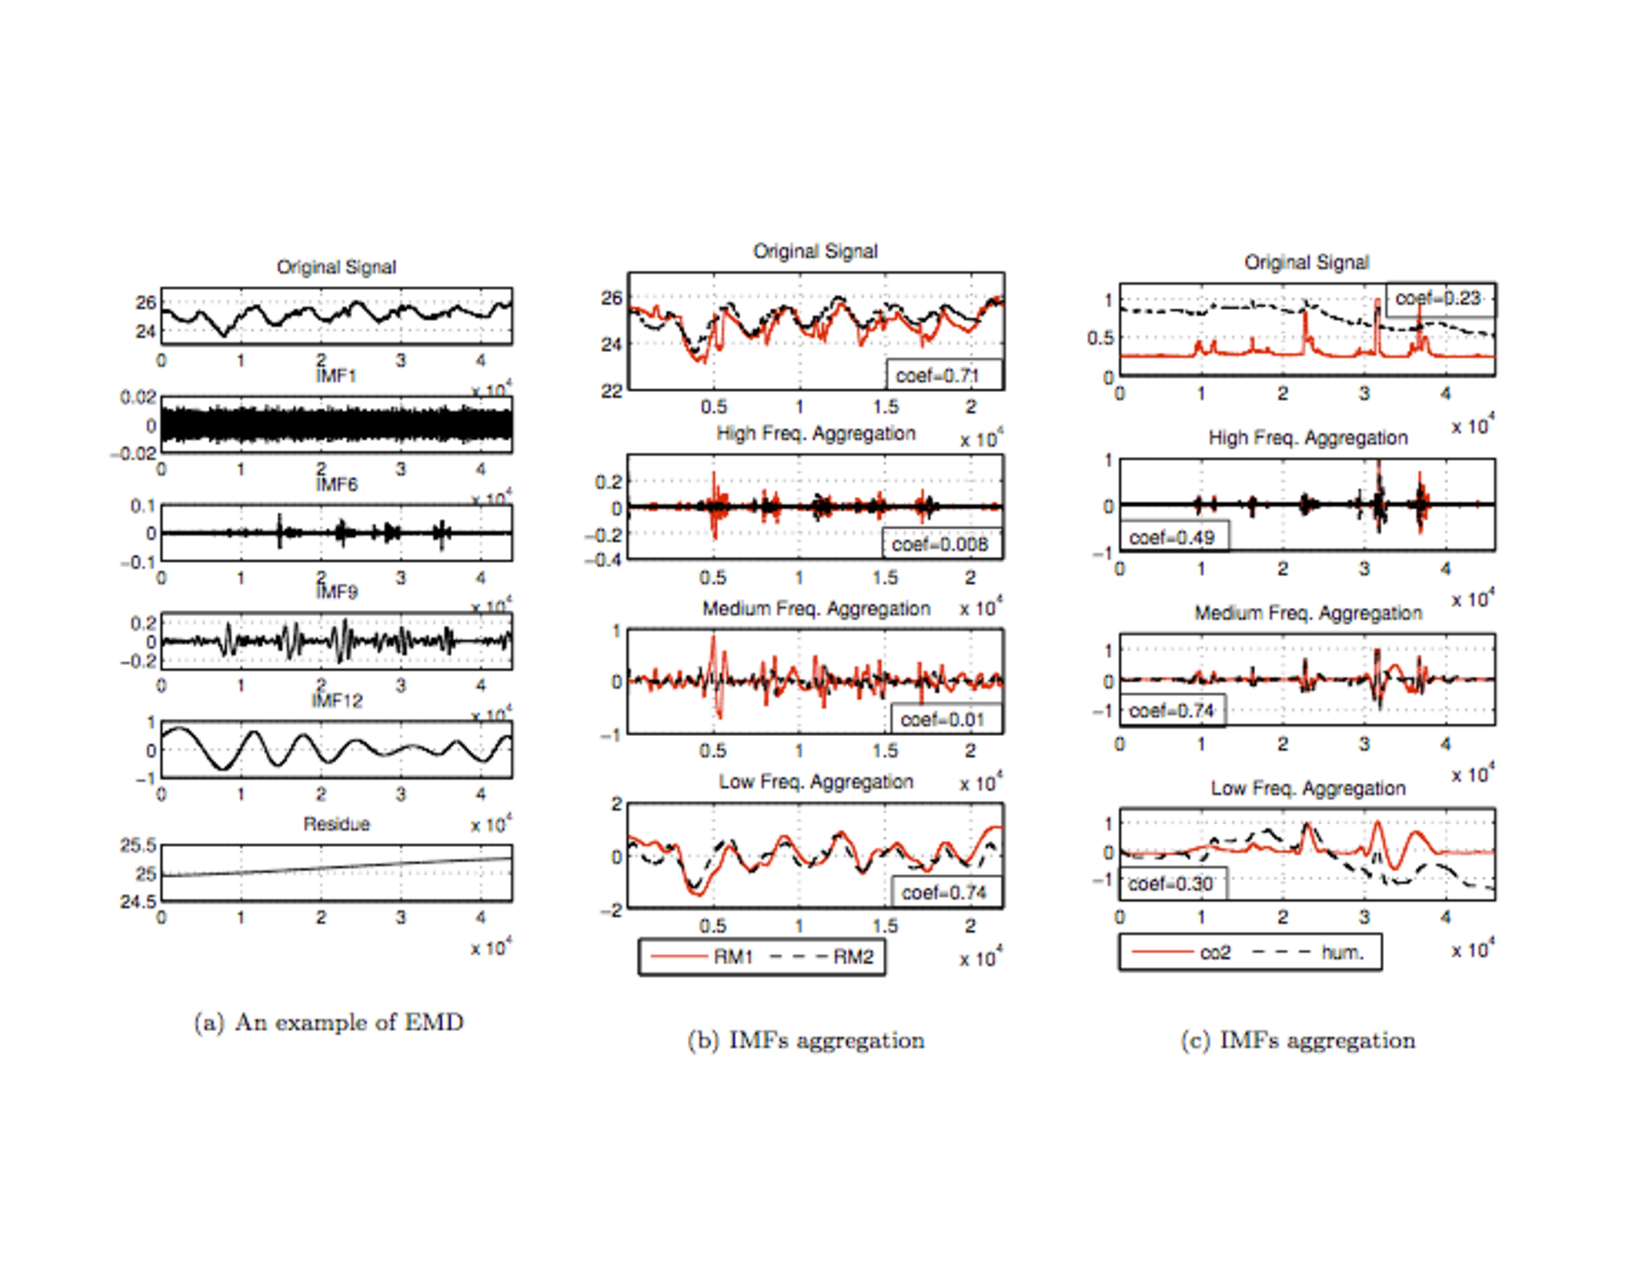
\includegraphics[width=0.95\textwidth]{figs/IMFReAggExample}
\caption{(a) EMD decomposes a signal and exposes intrinsic oscillatory components; (b) Aggregation of IMFs within a pre-defined frequency range makes seemingly similar signals from different locations more distinguishable; (c) IMF aggregation makes seemingly distinct signals of different sensors in the same room show high correlation.}
\end{figure*}

We start our analysis by extending the methodology used in SBS~\cite{SBS}, based on empirical mode decomposition (EMD).  
In our analysis, we collect traces from several sensors and run EMD on them.  This produces a set of 
constituent sub-signals called ``intrinsic mode functions'' (IMF), which we separate by frequency range and re-aggregate into distinct bands.
Then, we inspect the relationship between the sensors by computing the corrcoeff within a particular band, which 
gives us the spatial information we are interested in. 
Finally, we separate the result set into sub-sets, and closely examine their statistical characteristics. 
Before describing our methodology in detail, we introduce some definitions and notation.


\subsection{Correlation}
We make extensive use of the correlation coefficient function defined as: 

\begin{displaymath}
r(X,Y) = r_{X, Y} = \frac{\sum_{i=1}^{n} (X_{i} - \overline{X})(Y_{i} - \overline{Y})}
{\sqrt{\sum_{i=1}^{n} (X_{i} - \overline{X})^2}\sqrt{\sum_{i=1}^{n} (Y_{i} - \overline{Y})^2}}
\end{displaymath}

where $X$, $Y$ are separate sets of values, $n$ is the total number of sample points in 
each set, and $\overline{X}$ is the mean value of $X$ (same for $\overline{Y}$ and Y).  % over the entire sampling period.
For each pair of sensors, we compute the corrcoeff to ascertain the relationship between them.



\subsection{Type Verification}



\subsection{Value Verification}




